\chapter{Theoretical predictions and event simulation}
\label{ch:simulation}

Quantifying the agreement of experimental observations with the SM
or with possible BSM theories is a core goal of collider physics.
While the SM is a nearly complete and profoundly successful theory,
connecting theories which concern the interactions and excitations of quantum fields
to the electrical signals induced in the CMS detector by
\pp collisions is highly non-trivial.
In an ideal case, one would use
the theory of particles and fields outlined in Chapters~\ref{ch:introduction} 
and \ref{ch:phenomenology} as input to derive the expected distribution
of measurable signals resulting from \pp collisions.
In this paradigm, BSM modifications to the SM are realized as modifications 
to the structure of the underlying QFT. They lead to new interactions, which
modify the rate or type of particle production, or kinematics variables 
of the produced particles, leading to deviations from the SM expectation
in measured quantities. 
In practice, a factorized approach---leveraging approximations and tuning 
to experimental data---allows the simulation of primary particle production in
\pp collisions, the formation of bound states and particle decay,
and the interactions of particles in the CMS detector 
to be simulated in a way that largely achieves this goal.
The CMS Collaboration benefits from the work of collaborations of theoretical 
physicists and many previous studies to achieve detailed simulations.

It is important to highlight that the experimental physicists
is not purely at the mercy of the simulations from which our predictions derive.
Many predictions are phenomenological in nature, i.e., they have been tuned to the 
observations measured in LHC collisions and previous accelerators.
Furthermore, in situ measurements allow the data observation 
to modify aspects of the predictions. Lastly, broad knowledge of the nature
of particle production in collisions can sometimes be leveraged to completely 
remove dependence on simulation. For example, with no resonant source of 
diphoton production, the $m_{\gamma\gamma}$ distribution would be a falling spectrum.
The first measurements of the scalar Higgs boson with $m_{\PH} = 125\GeV$ made 
in the diphoton channel where achieved with the SM $\pp\to\gamma\gamma$ 
expectation parameterized as a falling exponential distribution,
not with an ab initio simulation of the distribution~\cite{Aad:2014eha,Khachatryan:2014ira}.

Nonetheless, the results presented in this thesis concern the measurement
of a rare SM process. In particular, determining the production mechanism
of {\WZjj} production and identifying the component that is sensitive to the
\WWZZ coupling relies heavily on achieving well-understood simulations of the
signal and background processes contributing to the events analyzed.
This chapter discusses the techniques used to simulate \pp collisions at the
LHC. The techniques used to obtain results for \WZjj production in the SM and beyond,
and the prediction used in this analysis, are presented. 
Their impact on the analysis and the role of the analysis in assessing the predictions
is discussed.

\section{Anatomy of an LHC collision}

As discussed in Chapter~\ref{ch:penomenology}, perturbation theory is the 
most effective technique for calculations of particle scattering in
the SM QFT. While the underlying principles are well-established, calculations
of QCD interactions, in particular, are computationally challenging. The QCD 
theory is asymptotically free, meaning $\alpha_s(\mu)$ grows with low values of 
the energy scale $\mu$, so low-energy phenomena are non-perturbative.
Because asymptotic freedom also leads to bound states at the low 
energy scales of most physical phenomena, the energy regime of stable particles---and
therefore the incoming state directed to collision and the outgoing particles
that interact with the detector---have non-perturbative properties.

The uncomfortable dichotomy between the regime of most physical phenomena and calculability
is averted by the concept of factorization, which allows a separation of short-distance
interactions from long-distance interactions, or equivalently, interactions governed
by energy scales large or small with respect to $\lqcd\approx 200\MeV$.
Factorization states that the interaction
of hadrons can be reduced to structure functions describing the distribution of quarks
and gluons in hadrons, known as parton distribution functions (PDF), convoluted
with the parton--parton interaction cross section. At high momentum transfer,
the parton--parton interaction can be described perturbatively. Furthermore,
the evolution of the interaction from outgoing quarks, gluons, and leptons
can be factorized from the formation of bound states, described by 
parton-to-hadron fragmentation functions, and their decay. The concept is illustrated
for \pp collisions in Fig.~\ref{fig:factorization}.
Factorization 
is formally established under certain conditions~\cite{Collins:1989gx}, and it 
has been highly successful in describing experimental observations over generations
of hadron--hadron, lepton--lepton, and hadron--lepton colliders.

\begin{figure}[htbp]
  \centering
   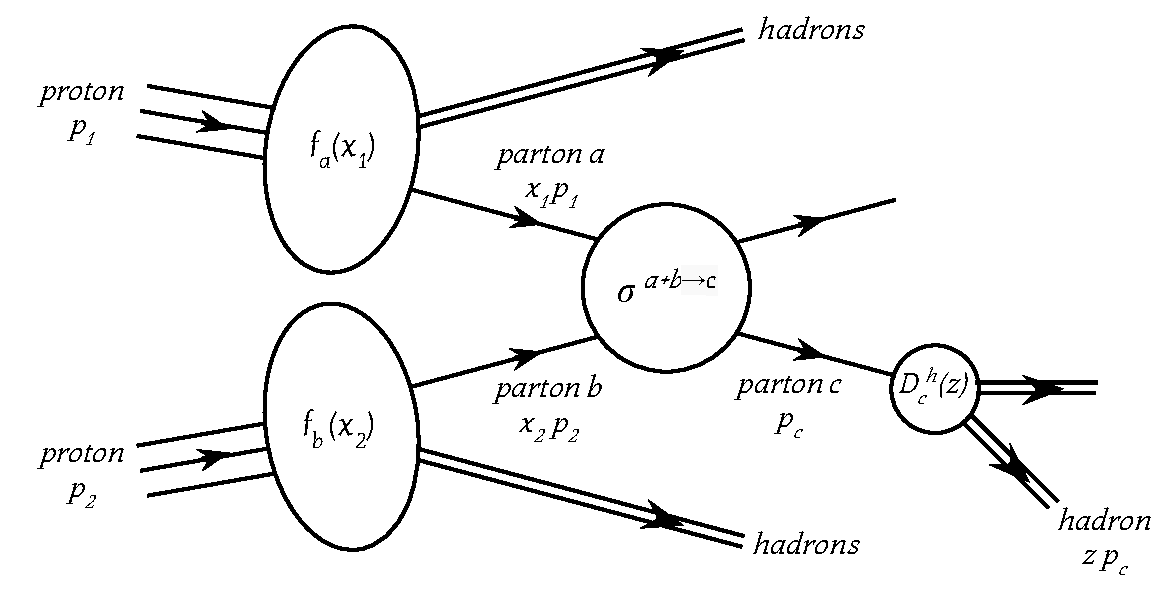
\includegraphics[width=0.6\textwidth]{figures/Simulation/factorization.pdf}
  \caption{
    Illustration of the principle of QCD factorization. The cross section
    of the process $\pp\to X$ is reduced to the parton distribution
    functions $f_{a,b}(x)$, the partonic cross sections $\sigma^{a+b\to c}$,
    and the parton-to-hadron fragmentation functions $D_{c}^{h}(z)$.
    Reproduced from Ref.~\cite{Adare:2014hsq}.
        }
 \label{fig:factorization}
\end{figure}


Factorization allows the challenge of describing LHC collisions to be
tackled in pieces, leveraging different techniques for each piece while benefiting
from possibly independent experimental data. 
This chapter summarizes how these factorized components are modeled
for the simulations that are used to guide in this analysis.
In some cases, it is useful to consider only some contributions.
For example, the effect of the experimental
reconstruction can be parameterized by reconstruction efficiencies, or the hadronization
of quarks and gluons can be reduced to an effective smearing, 
in cases where the effects are not dramatic and are well-established. 
Such predictions are also presented, and their relevance to this
analysis is discussed.

\section{Parton distribution functions}

One of the fundamental ideas of factorization is that the low-energy confinement
of quarks and gluons in the proton can be described independently from the 
parton--parton interaction in a hard collision, e.g., momentum transfer 
$Q^2 \gg \lqcd^2$. Mathematically, the 
separation of the proton structure and the high-$Q^2$ parton interaction,
shown pictorially in Fig.~\ref{fig:factorization}, can
be expressed as
\begin{equation}
  \sigma^{\pp\to X} = \sum_{a,b\in\{q,g\}}\int{\mathrm{d}x_1\mathrm{d}x_2f_{a}(x_1, \muF^{2})f_{a}(x_2,\muF^{2})}
      \hat{\sigma}^{\Pq\Pq'\to X}(x_1x_2s, \muF^{2})
\end{equation}
where $x_1$ and $x_2$ are the momentum fractions of the proton momentum carried by 
partons $a,b \in \{q,g\}$ and the PDFs $f_{a,b}(x_i)$ give
the probability of extracting the given parton with momentum fraction $x_{i}$.
The total momentum must be divided amongst the constituents, i.e.,
\begin{equation}
  \sum_{i}\int_{0}^{1}\mathrm{d}x xf_{i}(x, \muF^2) = 1
\end{equation}
Here $\muF$ is the factorization scale, an energy scale which represents the transition
from the non-perturbative regime of the PDF and the perturbative high $Q^2$ interaction.
Thought it is often convenient to take $\muF=Q^2$, $\muF$ is a free parameter that is an
artifact of the truncated serious in perturbation theory. As the order of the perturbation
expansion considered increases, the $\muF$ dependence of the result is reduced.

At least to very good approximation, the PDFs can be considered universal functions. 
Therefore, they can be derived using independent measurements, such as
deep inelastic scattering of lepton and proton beams. As shown in Fig.~\ref{fig:dis}, a lepton
incident on a proton target interacts with the quarks of the proton via a virtual
$\gamma$ or {\cPZ}. By controlling the incident energy of the proton and lepton and
measuring the outgoing particles the abundance and momentum fraction of the proton
constituents can be established.
\begin{figure}[htbp]
  \centering
   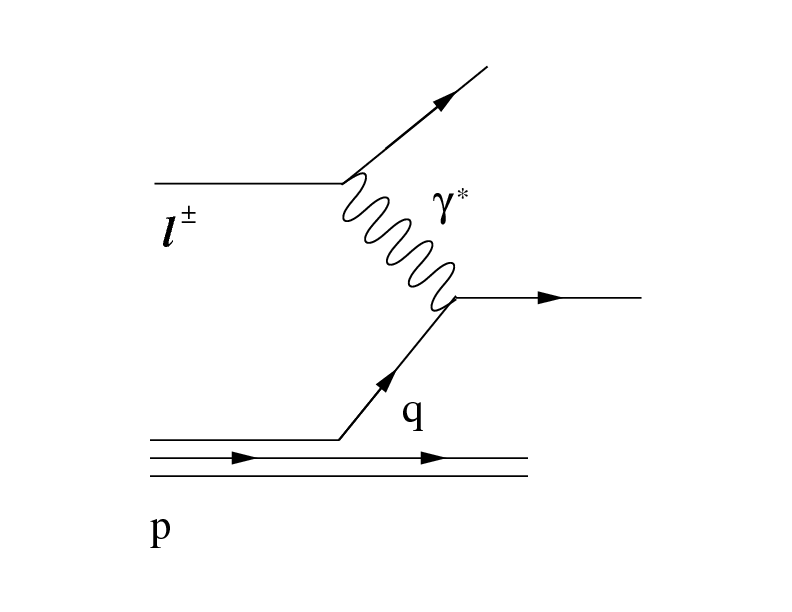
\includegraphics[width=0.4\textwidth]{figures/Simulation/DIS.png}
  \caption{
    Illustration of deep inelastic scattering of a lepton from a proton, used
    as a probe of the internal parton structure of the proton.
    Reproduced from Ref.~\cite{Filippone:2001ux}.
        }
 \label{fig:dis}
\end{figure}

In practice, it is not feasible to parameterize all partons (and flavors) for
all $x_{i}$ through experimental measurements. Fortunately, while perturbation theory
cannot predict the formation of bound states, it does allow a means to 
parameterize the evolution of the bound partons across energy scales. The scale
dependence of the PDF is captured by the DGLAP equations, first established
by Dokshitzer~\cite{Dokshitzer:1977sg}, Gribov~\cite{Gribov:1972ri}, 
Alterelli and Parisi~\cite{Altarelli:1977zs} in the 1970s:
\begin{equation}
  \muF^2\frac{\mathrm{d}f_{a}(x, \muF^2)}{\mathrm{d}muF^2} =
    \sum_{b\in\{q,g\}}\int_{x}^{1}\frac{\mathrm{d}z}{z}\frac{\alpha_s}{2\pi}
    \hat{P}_{ba}(z))f_b(x/z,\muF^2 \,.
\end{equation}
The functions $\hat{P}_{ba}(z)$ are the Alterelli--Parisi splitting functions,
which describe the splitting of parton $a$ into $b$, carrying a momentum
fraction $z$ of the initial momentum, that
can be derived order by order in perturbation theory. The splitting of
parton $a$ is accompanied by an additional parton, e.g., $\Pg\to\Pq\Paq$,
that is absorbed in to the parton sea of the proton. Given the DGLAP equations,
if the proton PDF can be established for any complete phase space of
parton flavors, momentum fractions, and $Q^2$, it can be evolved to all other 
scales. In practice, the contributions to the PDF are
at many different $Q^2$ with experiments sensitive to different quark flavors.
The experimental data is fitted, considering the DGLAP evolution, to obtain
a full parametrization of the PDF at all energy scales. 

Collaborations of theorist use independent techniques to fit data
from many collider and fixed target experiments to produce large data sets
of predictions that can be used in simulations. The PDF is parameterized
and distributed as data grids that can be sampled with a centralized interfaced
known as LHAPDF~\cite{Buckley:2014ana}. Results in this thesis primarily
make use of the NNPDF3.0~\cite{NNPDF2015} set of PDFs, which use a neutral net and generated
pseduodata to perform global fits to the data. 
Uncertainties in this procedure and their impact on this analysis 
are discussedin Chapter~\ref{ch:analysis}.
They are assessed by evaluating the quality of the PDF fit to the data, 
comparing the predictions of independent collaborations
in a formulaic way~\cite{Butterworth:2015oua}, and by determining
the dependence of predictions on $\muF$.

\section{Perturbative calculations and matrix element generators}

With the parton content of the proton captured by the PDFs, the next challenge
in modeling an LHC collision is the perturbative calculation of the parton--parton
interaction. As discussed in Chapter~\ref{ch:phenomenology}, perturbation theory
relies on an expansion in the coupling constants of the theory,
\begin{equation}
  \sigma = \sigma_0\alpha_s^{0} + \sigma_1\alpha_s^{1} + \sigma_2\alpha_s^{2} + \cdots\,.
  \label{eq:pqcd}
\end{equation}
For a process with only by EW couplings at the lowest order, such as VV production,
$\sigma_0 = \sigma_{LO}$ and $\sigma_1 = \sigma_{NLO}$.
While $\alpha_s$ is sufficiently small at the LHC collision energy to justify the
perturbative expansion ($\alpha_s(m_{\PZ}) = 0.1189 \pm 0.0010$~\cite{Tanabashi:2018oca}),
the energy and phase-space dependence of higher-order terms is non-trivial,
leading to QCD corrections much larger than the naive 
expectation in many cases~\cite{Altarelli:1979ub,Campbell:2011bn,Dittmaier:2011ti}.
The majority of production processes at the LHC require a calculation at least to NLO in QCD for percent-level accuracy.
Theoretical tools have advanced to allow automated computation of all 
SM processes at NLO~\cite{Gleisberg:2008ta,MGatNLO,Recola},
and many processes have recently been computed at NNLO in QCD~\cite{Grazzini:2017mhc}.
Calculations
at LO in the EW theory are often sufficient for percent-level accuracy. However,
some processes are susceptible to anomalously large EW corrections, including
VBS VV production~\cite{Biedermann:2016yds}, considered in this thesis.

The cross section of Equation~\ref{eq:pqcd} can be expressed in terms of the square of 
the scattering matrix element $\mathcal{M}$, which 
captures the transition probability from the initial to the final state.
The matrix element, or scattering amplitude, is calculable in perturbation theory, of which
techniques based on Feynman diagrams are the most familiar. 
Because the total cross section is a scan over all possible outgoing energy and momenta
combinations of the outgoing particles, the cross section is an integration over a
many-dimensional phase space of configurations $\Phi_{n}$,
\begin{equation}
  \sigma_{i} = \int \mathrm{d}\Phi_{n}\left|\mathcal{M}_i\right|^2 \,.
  \label{eq:meint}
\end{equation}
The integration can be performed with numerical techniques. The high dimensionality
of the phase space, as well as the complex peak structure arising from resonances,
is well-suited for Monte Carlo integration techniques, described in the following section.

In the Feynman diagram approach to matrix-element calculations, amplitudes are represented by Feynman diagrams
where QCD (EW) coupling vertices in the diagrams are proportional to $\sqrt{alpha_s}$ ($\alpha$).
A calculation at a given perturbative order involves all diagrams connecting 
desired initial and final states for which the product of vertices is less than the order
of the perturbative expansion.
Feynman diagrams can be generated in an automated procedure with techniques from graph theory, 
before being used to derive and calculate amplitudes from Feynamn rules in the SM.
Automation of this process was established in the early 1990s at LO~\cite{Stelzer:1994ta}.
Extending this to procedure to NLO has been accomplished more recently by the 
program \MG~\cite{MGatNLO}, the successor to the previous work, which is the used extensively
for results in this thesis.

Diagrams without loop contributions are called ``tree-level'' diagrams. The lowest tree-level
contribution to a given state, shown for $\pp\to\PW\PZ$ in Fig.~\ref{fig:WZNLO} (far left),
is referred to as the Born-level contribution to the process. The NLO correction to the Born
process includes contributions from tree-level diagrams of $\pp\to\PW\PZ+\jet$ for $\jet\in\{\Pg,\Pq\}$, 
known as real emission diagrams, and loop contributions, shown in Fig.~\ref{fig:WZNLO} (center)
and (left) respectively. 
Divergences from each of these contributions cancel through
renormalization. The delicate procedure of ``cancelling infinities'' via numerical techniques,
presents a major challenge to automating NLO calculations.
It requires a cut to be made precisely at the infinite pole, and 
careful management of the divergent contributions around the pole with high-precision numerical accuracy.
All possible one-loop amplitudes in the SM have been calculated with analytic techniques.
Automated codes access these loop contributions and residual divergences from packages such as
OpenLoops~\cite{Cascioli:2011va}, and combine them with the Born and real-emission calculations,
while verifying that the infinities of the loop and real-emission calculations do indeed cancel.
As the first NLO calculations became available, the interplay between contributions was
adjusted per process in dedicated calculations. For example in Refs. for the \WZ process
and Refs. for \EWWZ.
This procedure is now automated in several general-purpose MC programs, including
\MG~\cite{MGatNLO}, \Sherpa~\cite{Gleisberg:2008ta}, \Herwig~\cite{Bellm:2015jjp}, and \Recola~\cite{Recola}.
However, programs which automate all SM calculations are not optimized for specific
process, which can lead to prohibitively long computation time for high-multiplicity states
or processes with a complex phase, such as \EWWZ. For this reason, the best-available
calculations for the \QCDWZ and \EWWZ process come from dedicated implementations, such as
Refs.~\cite{Bozzi:2007ur,Campanario:2013qba}.

\begin{figure}[htbp]
  \centering
   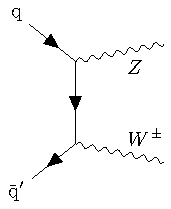
\includegraphics[page=1,width=0.22\textwidth]{figures/FeynmanDiagrams/WZNLOfeynman.pdf}
   \includegraphics[page=2,width=0.22\textwidth]{figures/FeynmanDiagrams/WZNLOfeynman.pdf}
   \includegraphics[page=3,width=0.22\textwidth]{figures/FeynmanDiagrams/WZNLOfeynman.pdf}
  \caption[Contributions to the $\pp\to\WZ$ process at NLO]{
    Contributions to the $\pp\to\WZ$ process at NLO. The leftmost diagram is the Born
    contribution, which is part of the LO calculation. The real-emission diagram
    is shown in the center, and the loop contribution is far right. The cross section
    is proportional to the square of the sum of amplitudes shown, which at 
    $\mathcal{O}(\alpha_s)$ includes the square of the Born and real-emission diagrams
    and the interference of the loop and Born diagrams.
  }
 \label{fig:WZNLO}
\end{figure}

Diboson processes inclusive in the number of jets have recently become available 
at next-to-next-to-leading order (NNLO)~\cite{Grazzini:2017mhc}. These calculations
have an additional layer of complication due to the more complex cancelling of
divergences between double loop, double real-emission, and combined real-emission
and loop contributions. They are not yet automated,
partially because not all two-loop amplitudes in the SM are known.
Combining these predictions with hadronization functions,
discussed in the following sections, is also not yet accomplished for diboson
processes. In this thesis, we use NNLO cross section calculations to 
correct the predicted yields of NLO simulations for diboson processes.

\section{Monte Carlo integration and event unweighting}

As referenced in the previous section, calculations of physical
quantities involve integrations of the amplitude over the relevant phase space
for the scattering process. Because the solution


The phase space integration in Equation~\ref{eq:meint}
is an integration over the quantum numbers and four-momenta of all particles 
considered. The integration is often complex and rarely solvable analytically.
Solutions can be obtained numerically, leveraging techniques which have
been widely studied in applied mathematics and computer science~\ref{}.
Because of the high-dimensionality of the integration, an algorithm 
for which the uncertainty scales independently of the dimensionality is highly 
desirable. For this reason, a technique based on random numbers known as 
Monte Carlo (MC) integration is used~\cite{doi:10.1002/wics.1314}. The algorithm
was first formally developed in the late 1940s as part of the Manhattan project,
with the name derived from the eponymous casino for due to its leveraging
of random processes~\cite{10.2307/2280232}.

The MC procedure estimates 
the integral of a function $f(x_{i},\cdots,x_n\equiv\vec{x})$, defined over a volume $V^{n}$,
is estimated by tossing random random points inside a known volume
over which the function is defined, of dimension $V^{n+1}$. The volume $V^{n+1}$
from which the random numbers are drawn must fully contain 
$f(\vec{x})$, however, no further knowledge of $f(\vec{x})$ over $V^{n+1}$ is required. The function
is evaluated for the coordinates $x_i\cdots x_n$ of the random point.
If the random point is inside the volume of $f(\vec{x})$, it is accepted,
if it falls in a region of $V^{n+1}$ outside of $f(\vec{x})$ it is rejected.
As the number of points sampled $N$ grows, the ratio of the number of accepted
points to $N$ times the volume of $V^{n+1}$ approaches the integral of $f(\vec{x})$.
This is illustrated for one dimension in Fig.~\ref{fig:mcintegration}.
The error of the integration decreases proportional to $\sqrt{N}$, which
is very poor for low dimension integration ($\lesssim$4) but much better than
traditional techniques for high-dimensional problems.

\begin{figure}[htbp]
  \centering
   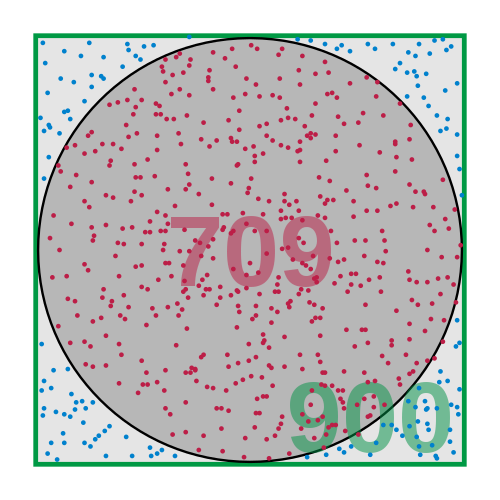
\includegraphics[width=0.6\textwidth]{figures/Simulation/MCintegration.png}
  \caption[Illustration of the principle of Monte Carlo integration.]{
    Illustration of the principle of Monte Carlo integration. If the area
    of the rectangular phase space is known, the area of the circle can
    be estimated from the ratio of randomly sampled points falling
    inside or outside the volume. In this example, the ratio of accepted
    points (709, red) to the total points sampled (900) approximates the
    analytic result for the ratio of the areas, $\pi/4$.
    Reproduced under public license from Ref.~\cite{wiki:mc}.
        }
 \label{fig:mcintegration}
\end{figure}

In addition to predictions for aggregated quantities such as total cross sections
and differential rates, event-wise simulations are critical to modeling expected 
results in the realistic environment of particle physics measurements.
The MC integration approach is well-suited for this, as the procedure of randomly
sampling the integrand over a phase space can be leveraged to draw events from
the distribution. In this procedure, specific realizations of particle states,
including quantum numbers and four momenta, are sampled from
the possible outcomes with rate proportional to the probability for production,
given by the phase space and squared amplitude of Equation~\ref{eq:meint}.

\section{Event simulation for experimental analysis}

Peturbation theory and matrix element calculations concern free
excitations of the fundamental
fields in the SM QFT. For the $\pp\to\WZ\to\ell\ell'\ell'\nu\jet\jet$ process, 
Equation~\ref{eq:meint} can be used to compute observables for the underlying
subprocesses, e.g., when a $\Pq\Pq'$ interaction takes place and
$\jet\jet=\Pq\Pq''$. This parton-level process can be used to derive useful predictions,
however, events containing free partons and leptons 
do not offer a full picture of the objects that interact with the CMS
detector. High-energy partons radiate quarks and gluons or split to quark--antiquark
pairs, reducing their energy until they reach the energy scale of hadronization \lqcd.
Similarly, leptons can radiate photons, which can subsequently pair produce photons.
Both effects are considered in the QCD and QED showers, which simulate successive soft
emissions of nearly-massless particles.
At the scale {\lqcd}, the free partons form hadrons. Long lived hadrons interact with the detector,
whereas shorter-lived hadrons decay to neutrinos, leptons, or other hadrons before interacting.
These considerations, combined with additional \pp interactions in a single LHC bunch crossing,
and multiple parton-parton in a single \pp collision, contribute to the full $\mathcal{O}(1000)$
particle multiplicity measured in the CMS detector per event. The properties and kinematic
distributions, as well as their interactions with the CMS detector, must be well-understood
for a full simulation of a realistic event.

\subsection{The parton shower and matching to matrix element calculations}
The shower allows radiations at low transverse momentum
and angular separation to be summed to all orders in perturbation theory, therefore populating

More generally, calculations at a fixed order in perturbation theory, as described in the proceeding
sections, have several shortcomings that must be accounted for when connecting
their predictions to physical measurements. Firstly, the fact that the perturbative
series has been truncated implies that higher-order effects are neglected. 
Measurements of quantities that are inclusive in the number of clustered partons associated
with the \WZ state may be have only a small dependence on these higher-order corrections.
However, the jets associated with the state have a strong dependence 


\subsection{The underlying event, hadronization, and decay}
Multiple parton-parton interatction
underlying event 
\subsection{Detector simulation}
\section{Predictions from fixed-order calculations}
\section{MC simulations of \WZjj production}

Here we present some of the studies done in comparison, quote the Les Houches paper,
and the paper on EW corrections, and yeah... Hopefully POWHEG
